% Primary figure
\begin{figure}[H]
    \centering
    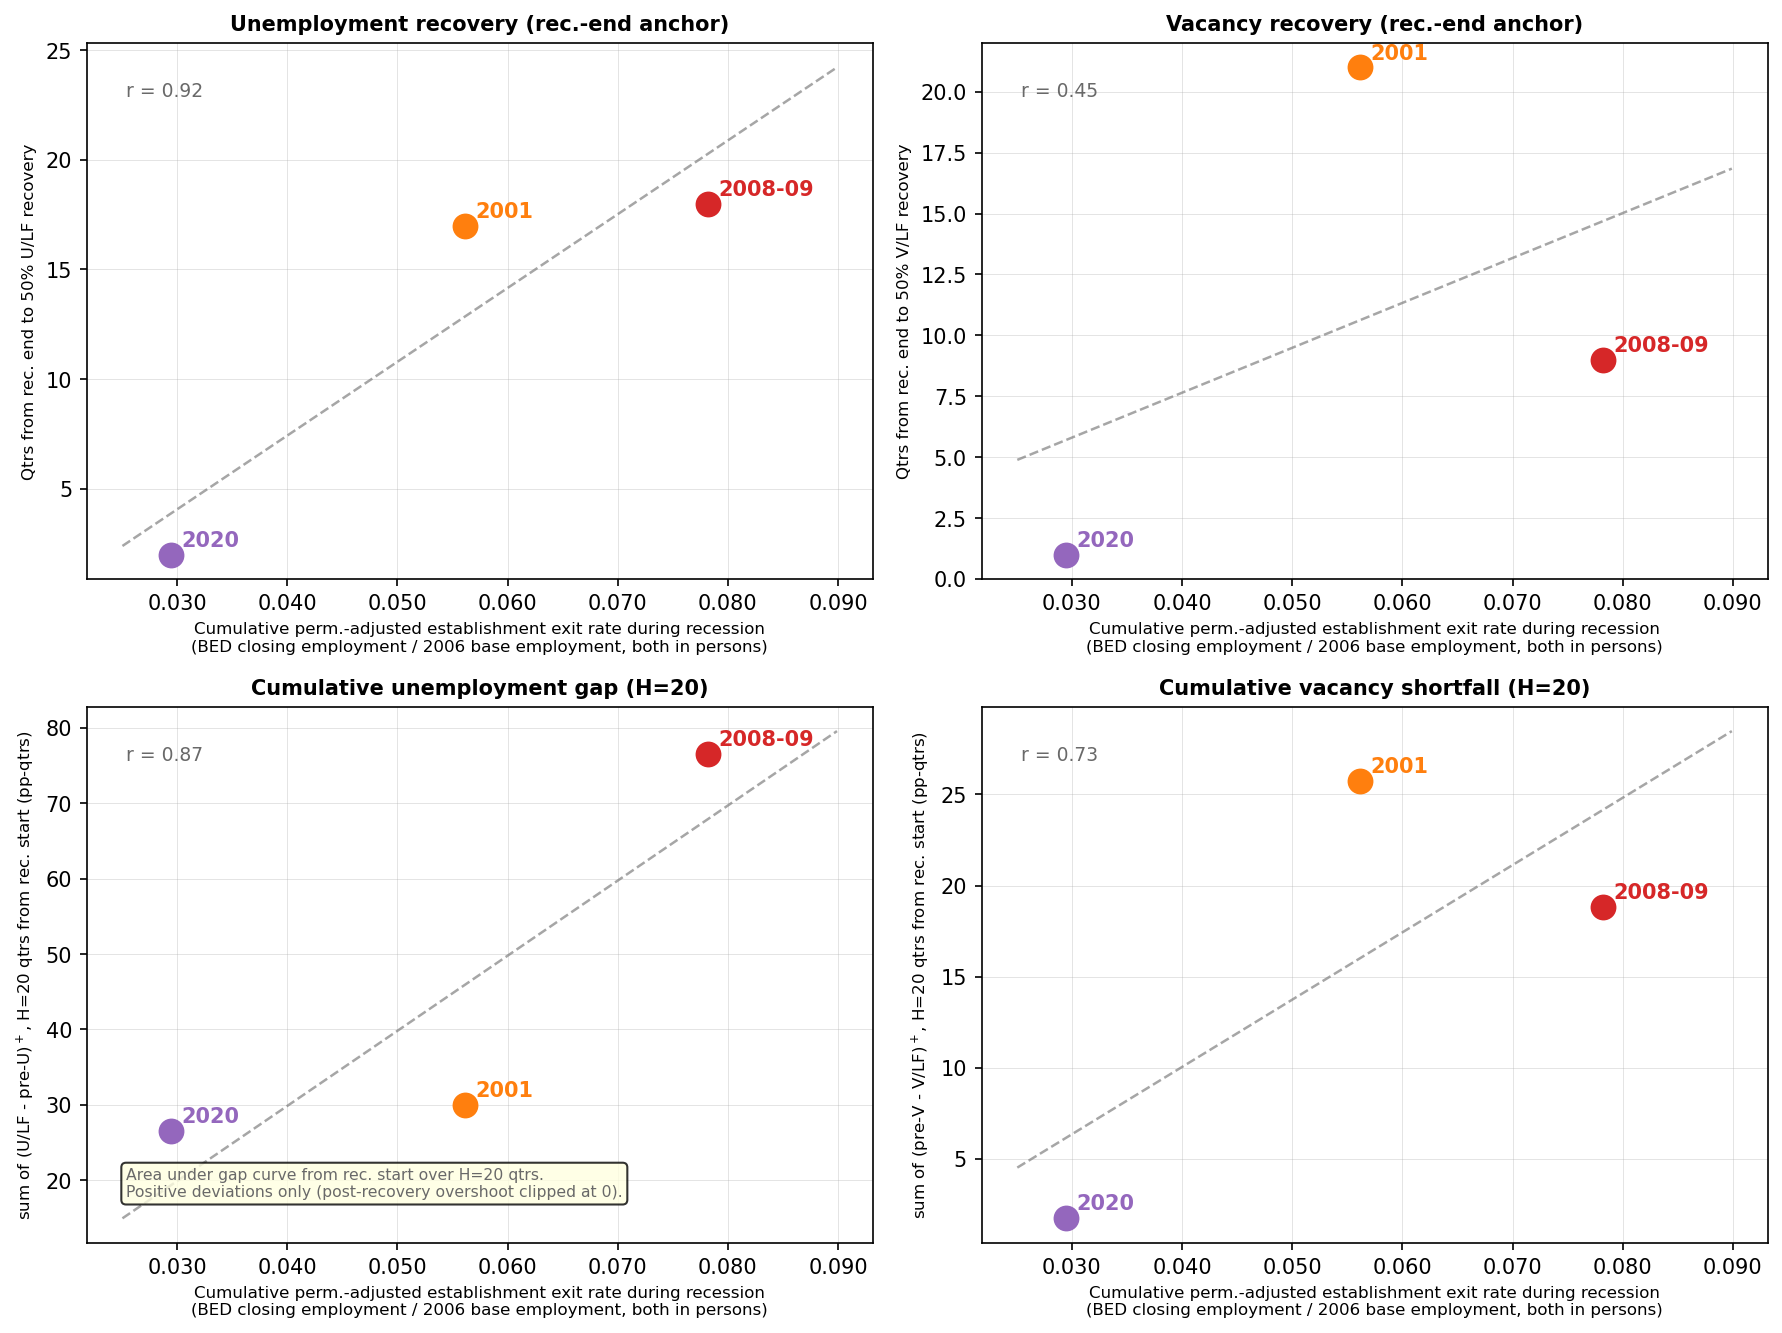
\includegraphics[width=0.9\textwidth]{recession_scatter_primary.png}
    \caption{Relationship between cumulative permanence-adjusted establishment
    exit rates during recessions and labor market outcome measures.
    The top row shows quarters from the NBER recession end date until
    unemployment (left) and vacancy (right) rates recover 50\% of the
    trough gap. The bottom row shows the cumulative unemployment gap
    (CUG, left) and cumulative vacancy shortfall (CVS, right), defined
    as the sum of positive deviations from the pre-recession baseline
    over $H=20$ quarters from recession onset. Exit rates are constructed
    from BLS Business Employment Dynamics (BED) establishment closing
    data, permanence-adjusted using Business Dynamics Statistics (BDS)
    death-to-closing ratios, and normalized by 2006 base-year employment.
    Vacancy data: Barnichon (2010) Composite Help-Wanted Index (pre-2001)
    spliced with JOLTS state-level job openings (2001 onward).
    Recessions: 2001, 2007--2009, 2020 (NBER dates).}
    \label{fig:recession_scatter_primary}
\end{figure}

% Appendix figure
\begin{figure}[H]
    \centering
    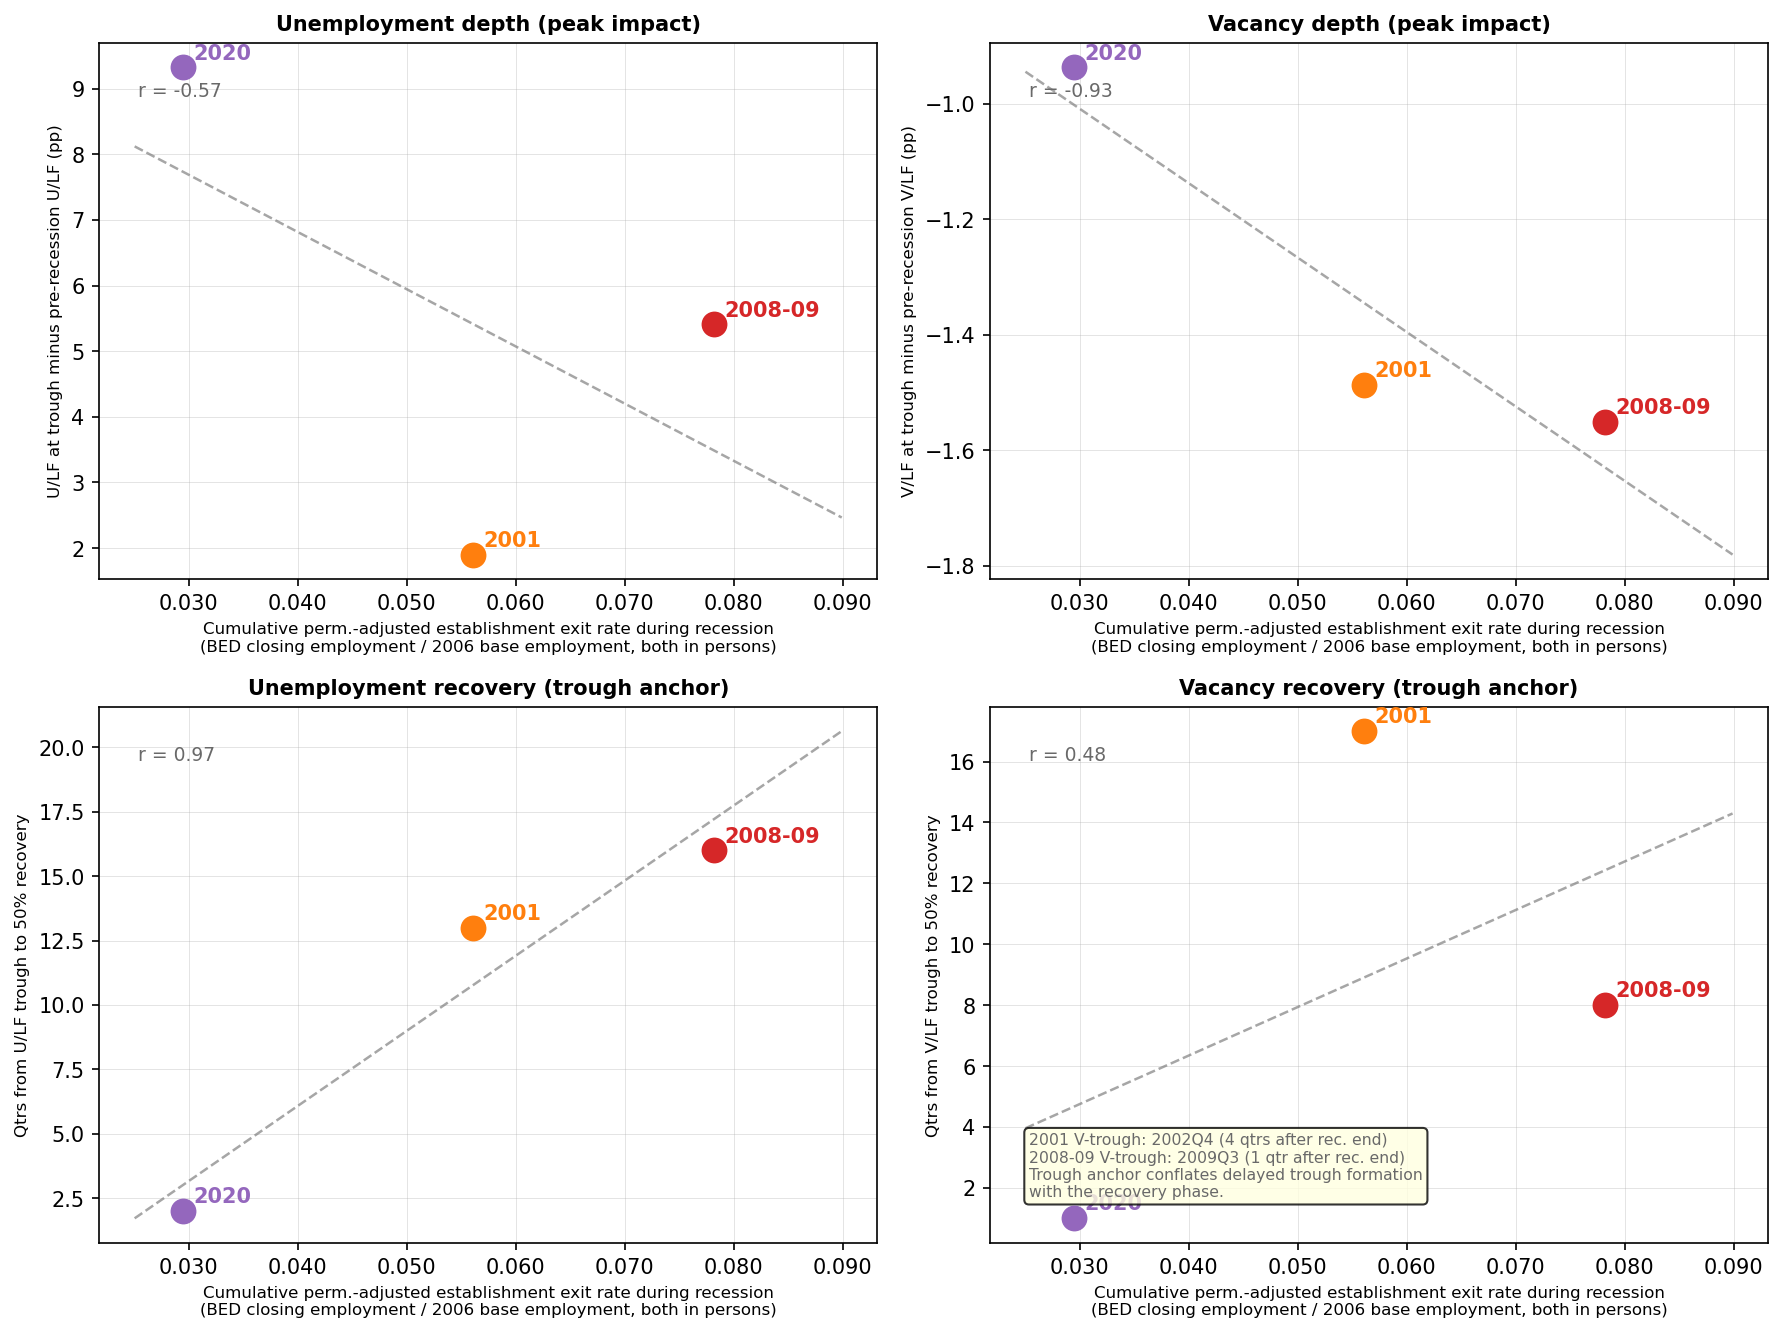
\includegraphics[width=0.9\textwidth]{recession_scatter_appendix.png}
    \caption{Supplementary recession severity measures.
    The top row shows the peak deviation of unemployment (left) and
    vacancy (right) rates from pre-recession baselines (percentage
    points). The bottom row shows quarters from the series trough
    until 50\% recovery for unemployment (left) and vacancies (right).
    Trough-anchored recovery times are sensitive to the lag between
    the NBER recession end date and the series nadir, which varies
    across episodes (2001 vacancy trough: 4 quarters after recession
    end; 2008--2009: 1 quarter). See Figure~\ref{fig:recession_scatter_primary}
    for data sources and construction details.}
    \label{fig:recession_scatter_appendix}
\end{figure}
